\subsection{Boundary tracking in CNLMs}
\label{sec:segmentation}

%    we used the same datasets for the full classifier and the one based on single units. In both cases, we could train them on 100 and 10k examples, for consistency? Or maybe just use 10k in all cases, explaining in the text why we use this size, and maybe even remarking that performance is well above chance also with much less data?

% The experiments in the previous sections rely on information that
% should be encoded in words, such as part of speech or agreement
% features.
The good performance of CNLMs on most tasks above suggests that,
although they lack a hard-coded word vocabulary and they were trained
on unsegmented input, there is enough pressure from the language
modeling task for them to learn to track word-like items, and
associate them with various morphological, syntactic and semantic
properties. In this section, we take a direct look at \emph{how} CNLMs
might be segmenting their input.
\newcite{Kementchedjhieva:Lopez:2018} found a \emph{single} unit in
their English CNLM that seems, qualitatively, to be tracking
morpheme/word boundaries.  Since they trained the model with
whitespace, the main function of this unit could simply be to predict
the very frequent whitespace character. We conjecture instead that the
ability to segment the input into meaningful items is so important
when processing language that CNLMs will specialize units for boundary
tracking even when trained without whitespace.

To look for ``boundary units'', we created a random set of 10,000
positions from the training set, balanced between those corresponding
to a word-final character and those occurring word-initially or
word-medially.  We then computed, for each hidden unit, the Pearson
correlation between its activations and a dummy variable coding
word-final position. For each language and model (LSTM or RNN), we
found very few units with a high correlation score, suggesting that
the models have indeed specialized units for boundary tracking. We
further study the units with the highest correlations, that are, for
the LSTMs, 0.58 (English), 0.69 (German), and 0.57 (Italian).
For the RNNs, the highest correlations are 0.40 (English), 0.46
(German and Italian).

We looked at the behaviour of the selected LSTM units qualitatively by
extracting random sets of 40-character strings from the development
partition of each language (left-aligned with word onsets) and
plotting the corresponding boundary unit activations. Figure
\ref{fig:word-unit} reports illustrative examples.  In all languages,
most peaks in activation mark word boundaries. However, other
interesting patterns emerge. In English, we see how the unit
reasonably treats \emph{co-} and \emph{produced} in \emph{co-produced}
as separate elements, and it also posits a weaker boundary after the
prefix \emph{pro-}. As it proceeds
left-to-right, with no information on what follows, the network posits a boundary after \emph{but} in \emph{Buttrich}. In
the German example, we observe how the complex word
\emph{Hauptaufgabe} is segmented into the morphemes \emph{haupt},
\emph{auf} and \emph{gabe}. Similarly, in the final
\emph{transformati-} fragment, we observe a weak boundary after the prefix
\emph{trans}. In Italian, \emph{in seguito a} is a lexicalized
multi-word sequence meaning `following' (literally: `in
continuation to'). The boundary unit does not spike inside
it. Similarly, the fixed expression \emph{Sommo Pontefice} (referring
to the Pope) does not trigger inner boundary unit activation spikes.  On the
other hand, we notice peaks after \emph{di} and \emph{mi} in
\emph{dimissioni}. Again, in left-to-right processing, the unit has a
tendency to immediately posit boundaries when frequent function words
are encountered.

% English /home/user/CS_SCR/FAIR18/CHECKPOINTS/boundary-neuron//
% Italian /home/user/CS_SCR/FAIR18/CHECKPOINTS/boundary-neuron//
% German /home/user/CS_SCR/FAIR18/CHECKPOINTS/boundary-neuron//

\begin{figure*}
  \begin{center}
  % \includegraphics[width=0.9\textwidth]{figures/{english_wiki-english-nospaces-bptt-282506230_15.txt}.png}
  \includegraphics[width=0.9\textwidth]{figures/{sent_english_wiki-english-nospaces-bptt-282506230_145.txt}.png}
  \includegraphics[width=0.9\textwidth]{figures/{german_wiki-german-nospaces-bptt-910515909_12.txt}.png}
  % \includegraphics[width=0.9\textwidth]{figures/{italian_wiki-italian-nospaces-bptt-855947412_7.txt}.png
  \includegraphics[width=0.9\textwidth]{figures/{sent_italian_wiki-italian-nospaces-bptt-855947412_301.txt}.png}
  \end{center}
  \caption{Examples of the LSTM CNLM boundary unit activation profile, with ground-truth word boundaries marked in
    green. English: \emph{It was co-produced with Martin Buttrich over at\ldots}. German: \emph{Systeme, deren Hauptaufgabe die transformati(-on)} `systems, whose main task is the transformation\ldots'. Italian: \emph{in seguito alle dimissioni del Sommo Pontefice} `following the resignation of the Supreme Pontiff\ldots'. \textbf{Is there a need to clean up the English and Italian
      plots? You mentioned adding manual word boundaries?}}\label{fig:word-unit}
\end{figure*}

To gain a more quantitative understanding of how well the boundary
unit is tracking word boundaries, we trained a single-parameter
diagnostic classifier on the activation of the unit (the classifier
simply sets an optimal threshold on the unit activation to separate
word boundaries from word-initial/internal positions). To train and
test the classifier, we randomly selected positions from the
development partition such that half of these were the last character
of a token, and the other half were not.  We collected 1,000 such
points as training data for the diagnostic classifiers, and used the
remainder for testing.  Both sets were balanced between (1) and (2).
We sampled the test data points subject to the constraint that the
word or word prefix ending at the selected character does not overlap
with the training set.  This ensures that a classifier cannot succeed
by looking for encodings reflecting specific words. \textbf{Please
  clarify this paragraph: What is the classifier fed, exactly? What is
  the development partition? Why the development one and not the test
  one?  What is the size of the reminder? What are (1) and (2)? What
  is the size of the substring fed to the classifier?  Finally,
  provide example for the last point.} As a reference point, we
moreover train a diagnostic classifier on the \emph{full} hidden layer
of the LSTMs.

Results are shown in Table~\ref{tab:segmentation-results}. The
LSTM-based full-hidden-layer classifier shows strong performance in
all 3 languages, confirming that the model encodes information about
boundaries. Moreover, in all languages, a large proportion of the full
performance is already accounted for by the single-parameter
classifier using boundary unit activations (the latter even
out-performs the full classifier in German). This confirms that
tracking boundaries is important enough for the network to devote a
specialized unit to this task. %
%(first, second and last
% columns). Performance of the LSTM CNLM closely matches that of the
% strong lexicon-based control, suggesting that the model is largely
% able to keep track of word boundaries.
Indeed, the single-unit LSTM classifier outperforms the full-layer RNN
classifier in all languages. RNN performance, while still much higher
than chance, is lagging behind. The overall weaker performance of RNNs
in the word-centric tasks of the previous sections might in part be
due to their poorer ability to track word boundaries. %

\begin{table}[t]
	\small
  \begin{center}
    \begin{tabular}{l|l|l|l|l|}
      \multicolumn{1}{c|}{}&\emph{LSTM}&\emph{RNN}&\emph{LSTM}&\emph{RNN}\\
            \multicolumn{1}{c|}{}&\emph{single}&\emph{single}&\emph{full}&\emph{full}\\
      \hline
      English & 77.5 & 65.6 & 89.9 & 76.8\\ 
      German  & 80.8 & 66.8 & 79.8 & 75.8\\ 
      Italian & 75.4 & 71.6 & 83.0 & 75.9\\ 
    \end{tabular}
  \end{center}
  \caption{\label{tab:segmentation-results} Accuracy of word boundary diagnostic classifiers trained on single boundary unit or full hidden state. Chance accuracy is at 50\%.}
\end{table}

% \begin{table}[t]
% 	\small
%   \begin{center}
%     \begin{tabular}{l|l|l||l}
%       \multicolumn{1}{c|}{}&\emph{LSTM}&\emph{RNN}&\emph{LSTM} with whitespace\\
%       \hline
% 	    English & 77.5 & 65.6 & 83.2 \\ 
% 	    German & 80.8 & 66.8  & 71.3  \\ 
% 	    Italian & 75.4 & 71.6 & 78.1 \\ 
%     \end{tabular}
%   \end{center}
%   \caption{\label{tab:segmentation-unit-results} Accuracy of threshold classifier based on `word' unit in distinguishing word boundaries from word-internal positions. Random baseline accuracy is 50 \%.}
% \end{table}


%
%\begin{table}[t]
%	\small
%  \begin{center}
%    \begin{tabular}{l|l|l|l}
%      \multicolumn{1}{c|}{}&\emph{LSTM}&\emph{RNN}&\emph{Lexicon}\\
%      \hline
%      English & 72.7/89.9/91.8 &  66.6/76.8/84.5  &  88.7   \\ 
%      German & 61.8/79.8/87.6  &  61.5/75.8/84.3 &  79.3  \\ 
%      Italian &  60.7/83.0/90.2 &  69.1/75.9/86.6  &  84.2   \\ 
%    \end{tabular}
%  \end{center}
%  \caption{\label{tab:segmentation-results} Accuracy of diagnostic classifier on recognizing word boundaries, with 100/1000/10000 training samples. Random baseline accuracy is 50 \%.}
%\end{table}
%Note that the models can have further 
%For LSTM CNLMs, we found at least 5 units with strong correlations ($>0.5$). For the RNN CNLMs, we also found at least one unit with correlation $> 0.4$ in each of the languages.

% \begin{table}[t]
% 	\small
%   \begin{center}
%     \begin{tabular}{l|l|l||l}
%       \multicolumn{1}{c|}{}&\emph{LSTM}&\emph{RNN}&\emph{LSTM} with whitespace\\
%       \hline
% 	    English & 77.5 & 65.6 & 83.2 \\ 
% 	    German & 80.8 & 66.8  & 71.3  \\ 
% 	    Italian & 75.4 & 71.6 & 78.1 \\ 
%     \end{tabular}
%   \end{center}
%   \caption{\label{tab:segmentation-unit-results} Accuracy of threshold classifier based on `word' unit in distinguishing word boundaries from word-internal positions. Random baseline accuracy is 50 \%.}
% \end{table}

As a final way to characterize the function and behaviour of the
boundary units, we inspected the most frequent under- and
over-segmentation errors made by the classifier based on them. We
discuss German here, as it is the language where the classifier
reaches highest accuracy, and its tendency to have long,
morphologically complex words makes it particularly
interesting. However, similar patterns were also detected in Italian
and, to a lesser extent, English (in the latter, there are fewer and
less interpretable common oversegmentations, probably because words are
on average shorter and morphology more limited).

Considering first the 30 most common undersegmentations, the large
majority (24/30) are common sequences of grammatical terms or very
frequent items that can sometimes be reasonably be re-analyzed as
single function words or adverbs (e.g., \emph{bis zu}, `up to'
(lit.~`until to'), \emph{je nach} `depending on' (lit.~`per after'),
\emph{bis heute} `to date' (lit.~'until today'). 3 cases are
multi-word city names (\emph{Los Angeles}). The final 3 cases
interestingly involve \emph{Bau} `building' followed by \emph{von}
`of' and genitive determiners \emph{der/des}. In its eventive reading,
this noun requires a patient licensed by either a preposition or the
genitive determiner, e.g., \emph{Bau der Mauer} `building of the wall'
(lit.~'building the-GEN wall'). Apparently the model decided to absorb
the case assigner into the form of the noun.

We looked next at the 30 most common oversegmentations, that is, at the
 substrings that were wrongly segmented out of the largest
number of distinct words. We limited the analysis to those containing
at least 3 characters, because shorter strings were ambiguous and
hard to interpret. Among then top oversegmentations, 6 are prefixes that can also occur in
isolation as prepositions or verb particles (\emph{auf} `on',
\emph{nach} `after', etc.). 7 are content words that form many
compounds (e.g., \emph{haupt} `main', occurring in \emph{Hauptstadt}
`capital', \emph{Hauptbahnhof} `main station' etc.; \emph{Land}
`land', occurring in \emph{Deutschland} `Germany', \emph{Landkreis}
`district', etc.). Another 7 items can be classified as suffixes
(e.g., \emph{-lich} as in \emph{s\"udlich} `southern',
\emph{wissenschaftlich} `scientific'), although their segmentation is
not always canonical (e.g., \emph{-chaft} instead of the expected
\emph{-schaft} in \emph{Wissenschaft} `science'). 4 very common
function words are often wrongly segmented out of longer words (e.g.,
\emph{sie} `she' from \emph{sieben} `seven'). The \emph{kom} and
\emph{kon} cases are interesting, as the model
reasonably segment them as stems in forms of the verbs \emph{kommen} `to
come' and \emph{kennen} `to know', respectively (e.g., \emph{kommt}
and \emph{konnte}), but it also treats them as pseudo-prefixes elsewhere
(\emph{komponist} `composer', \emph{kontakt} `contact'). The remaining
3 oversegmentations, \emph{rie}, \emph{run} and \emph{ter} don't have
any clear interpretation.

Our analyses highlight the fact that the boundary unit, even when
analyzed through the lens of a classifier that was optimized on
word-level segmentation, is actually tracking salient linguistic
boundaries at different levels. While in many cases these boundaries
naturally coincide with words (hence the high classifier performance),
the CNLM is also sensitive to frequent morphemes and compound
elements, as well as to different types of multi-word
expressions. This is in line with a view of wordhood as a useful but
``soft'', emergent property, rather than a rigid primitive of
linguistic processing.

% python detectBoundariesUnit_Hidden_ExtractPattern_NoWhitespace_Classifier.py --language english  --batchSize 128 --char_dropout_prob 0.001 --char_embedding_size 200 --char_noise_prob 0.0 --hidden_dim 1024 --language english --layer_num 3 --learning_rate 3.6  --myID 282506230 --load-from wiki-english-nospaces-bptt-282506230 --weight_dropout_hidden 0.01 --weight_dropout_in 0.0
% output in 
% results/segmentation-english-frequent-errors-unit-disjoint.txt



% OLD FROM HERE



% In this section, we look
% directly at whether the hidden state of the CNLMs is directly
% sensitive to word boundaries, when processing unsegmented
% input. First, using the method of diagnostic classifiers, we check
% whether we can decode word boundaries from the whole hidden activation
% vectors of pre-trained CNLMs that is reading new input. Next, we focus
% on \emph{single hidden units} that, in all studied languages, seem to
% have specialized on tracking boundaries.

% We randomly selected positions from the development partition such
% that half of these were the last character of a token, and the other
% half were not.  We collected 1,000 such points as training data for
% the diagnostic classifiers, and the remainder for testing.  Both sets
% were balanced between (1) and (2).  We sampled the test data points
% subject to the constraint that the word or word prefix ending at the
% selected character does not overlap with the training set.  This
% ensures that the diagnostic classifier cannot succeed by looking for
% encodings reflecting specific words. \textbf{Please clarify this
%   paragraph: What is the classifier fed, exactly? What is the
%   development partition? Why the development one and not the test one?
%   What is the size of the reminder? What are (1) and (2)? Finally,
%   provide example for the last point.}

% For a performance reference point, we trained the following control
% lexicon-based classifier.  Given a position where the last word is
% $x_1...x_n$ \textbf{(did not understand this)}, we count how often
% $x_1...x_n$ occurs as a token in the tokenized Wikipedia training set
% ($N_1$), and how often a longer word starting with $x_1...x_n$ occurs
% there ($N_2$).  The classifier guesses that a boundary is present if
% $N_1 > N_2$, no boundary if $N_1 < N_2$, and randomly if $N_1 =
% N_2$. \textbf{Give one example.}  This is a very strong classifier:
% First, unlike the CNLM, it has oracle access to the beginning of the
% current word.  Thus, it is the \emph{optimal} classifier when the
% beginning of the current word is known, but prior context is not
% given. \textbf{Please explain previous point, I didn't get it.}
% Furthermore, it has access to a very large lexicon listing all unigram
% counts in the training corpus, encoding a vast amount of lexical
% knowledge.

% Results are shown in Table~\ref{tab:segmentation-results} (first,
% second and last columns). Performance of the LSTM CNLM closely matches
% that of the strong lexicon-based control, suggesting that the model is
% largely able to keep track of word boundaries. The RNN performance,
% while still much higher than chance, is lagging behind The overall
% weaker performance of this model in the word-centric tasks of the
% previous sections might in part be due to its poorer ability to track
% words. %
% %, and outperforms it with 10,000 training samples.
% %We find that the diagnostic classifier shows above-random performance with few training samples, though its performance lags behind that of the single-parameter classifiers derived from the units we found above, suggesting overfitting of the diagnostic logistic classifier.
% %With 1000 training samples, the diagnostic classifier performs similarly to the strong lexicon-based classifier. %, and outperforms it with 10,000 training samples.
% % This shows that the CNLM's representations provide strong cues regarding word boundaries.
% % Performance is strongest in English and weakest in German, both for the CNLM-based diagnostic classifier and for the lexicon-based baseline.
% % The preponderance of compound words in German may be responsible for this.
% Note that, overall, English is the easiest language. We conjecture
% that this is related to the fact that CNLMs might be tracking useful
% linguistic boundaries, that might sometimes delimit morphemes or
% compound elements, rather than words. As our evaluation is instead
% (for practical reasons) strictly word-based, the more morphologically
% rich languages are negatively affected (we will return to this point
% below).

% % \begin{table}[t]
% % 	\small
% %   \begin{center}
% %     \begin{tabular}{l|l|l|l}
% %       \multicolumn{1}{c|}{}&\emph{LSTM}&\emph{RNN}&\emph{Lexicon}\\
% %       \hline
% %       English & 89.9 &  76.8  &  88.7   \\ 
% %       German & 79.8  &  75.8 &  79.3  \\ 
% %       Italian &  83.0 &  75.9  &  84.2   \\ 
% %     \end{tabular}
% %   \end{center}
% %   \caption{\label{tab:segmentation-results} Accuracy of word boundary diagnostic classifiers trained on full hidden state or on single 'boundary' unit, plus lexicon-based control. Chance accuracy is at 50\%.}
% % \end{table}


% \begin{table}[t]
% 	\small
%   \begin{center}
%     \begin{tabular}{l|l|l|l|l||l}
%       \multicolumn{1}{c|}{}&\emph{LSTM}&\emph{RNN}&\emph{LSTM}&\emph{RNN}&\emph{Lex.}\\
%             \multicolumn{1}{c|}{}&\emph{full}&\emph{full}&\emph{single}&\emph{single}&\\
%       \hline
%       English & 89.9 &  76.8  & 77.5 & 65.6&  88.7   \\ 
%       German & 79.8  &  75.8  & 80.8 & 66.8& 79.3  \\ 
%       Italian &  83.0 &  75.9 & 75.4 & 71.6&  84.2   \\ 
%     \end{tabular}
%   \end{center}
%   \caption{\label{tab:segmentation-results} Accuracy of word boundary diagnostic classifiers trained on full hidden state or on single 'boundary' unit, plus lexicon-based control (Lex.). Chance accuracy is at 50\%.}
% \end{table}

% % \begin{table}[t]
% % 	\small
% %   \begin{center}
% %     \begin{tabular}{l|l|l||l}
% %       \multicolumn{1}{c|}{}&\emph{LSTM}&\emph{RNN}&\emph{LSTM} with whitespace\\
% %       \hline
% % 	    English & 77.5 & 65.6 & 83.2 \\ 
% % 	    German & 80.8 & 66.8  & 71.3  \\ 
% % 	    Italian & 75.4 & 71.6 & 78.1 \\ 
% %     \end{tabular}
% %   \end{center}
% %   \caption{\label{tab:segmentation-unit-results} Accuracy of threshold classifier based on `word' unit in distinguishing word boundaries from word-internal positions. Random baseline accuracy is 50 \%.}
% % \end{table}


% %
% %\begin{table}[t]
% %	\small
% %  \begin{center}
% %    \begin{tabular}{l|l|l|l}
% %      \multicolumn{1}{c|}{}&\emph{LSTM}&\emph{RNN}&\emph{Lexicon}\\
% %      \hline
% %      English & 72.7/89.9/91.8 &  66.6/76.8/84.5  &  88.7   \\ 
% %      German & 61.8/79.8/87.6  &  61.5/75.8/84.3 &  79.3  \\ 
% %      Italian &  60.7/83.0/90.2 &  69.1/75.9/86.6  &  84.2   \\ 
% %    \end{tabular}
% %  \end{center}
% %  \caption{\label{tab:segmentation-results} Accuracy of diagnostic classifier on recognizing word boundaries, with 100/1000/10000 training samples. Random baseline accuracy is 50 \%.}
% %\end{table}

% \newcite{Kementchedjhieva:Lopez:2018} found a unit in their English
% CNLM that seems to be tracking morpheme/word boundaries.  Since they
% trained the model with white space, it might have had a strong
% pressure to develop such unit in order to predict the very frequent
% white space character. Do our models, who don't have this direct
% pressure, also specialize units for boundary tracking, or is the
% information detected by our classifier opaquely stored in the
% full distributed hidden state?

% To look for boundary units, we created a random set of 10,000
% positions from the training set, balanced between those corresponding
% to a word-final character and those occurring word-initially or
% word-medially.  We then computed, for each hidden unit, the Pearson
% correlation between its activations and a dummy variable coding
% word-final position. For each language and model (LSTM and RNN), we
% found very few units with a high correlation score, suggesting that
% the models have indeed specialized units for boundary tracking. We
% further study the units with the highest correlations, that are, for
% the LSTM CNLMS, at 0.58 (English), 0.69 (German), and 0.57 (Italian).
% For the RNN CNLMs, the highest correlations were 0.40 (English), 0.46
% (German and Italian).
% %Note that the models can have further 
% %For LSTM CNLMs, we found at least 5 units with strong correlations ($>0.5$). For the RNN CNLMs, we also found at least one unit with correlation $> 0.4$ in each of the languages.

% To gauge insights on the behaviour of the selected LSTM CNLM units, we
% extracted random sets of 40-character strings from the development
% partition of each language (constrained to start word-initially) and
% plotted the corresponding `boundary unit' activations. Figure
% \ref{fig:word-unit} reports illustrative examples.  In all languages,
% peaks in activation do indeed tend to mark word boundaries. However,
% other interesting patterns emerge. In English, we see how the unit
% reasonably treats \emph{co-} and \emph{produced} in \emph{co-produced}
% as separate elements, and it also posits weaker boundaries after the
% prefix \emph{pro-} and the suffix \emph{-d}. As it proceeds
% left-to-right, with no information on what follows, the network seems
% to predict a boundary after \emph{but} in the last \emph{Buttrich}. In
% the German example, we observe how the complex word
% \emph{Hauptaufgabe} is segmented into the morphemes \emph{haupt},
% \emph{auf} and \emph{gabe}. Similarly, in the final
% \emph{transformati-} fragment, we observe a weak boundary after prefix
% \emph{trans}. In Italian, \emph{In seguito a-} is a lexicalized multi-word
% sequence meaning ``following'' (literally: ``in continuation
% to''). The boundary unit does not spike inside it. Similarly, the
% fixed expression \emph{Sommo Pontefice} (referring to the Pope) does
% not show boundary unit activation spikes.  On the other hand, we
% notice peaks after \emph{di} and \emph{mi} in
% \emph{dimissioni}. Again, in left-to-right processing, the unit has a
% tendency to immediately posit boundaries when frequent function words
% are encountered.

% % English /home/user/CS_SCR/FAIR18/CHECKPOINTS/boundary-neuron//
% % Italian /home/user/CS_SCR/FAIR18/CHECKPOINTS/boundary-neuron//
% % German /home/user/CS_SCR/FAIR18/CHECKPOINTS/boundary-neuron//

% \begin{figure*}
%   % \includegraphics[width=0.9\textwidth]{figures/{english_wiki-english-nospaces-bptt-282506230_15.txt}.png}
%   \includegraphics[width=0.9\textwidth]{figures/{sent_english_wiki-english-nospaces-bptt-282506230_145.txt}.png}
%   \includegraphics[width=0.9\textwidth]{figures/{german_wiki-german-nospaces-bptt-910515909_12.txt}.png}
%   % \includegraphics[width=0.9\textwidth]{figures/{italian_wiki-italian-nospaces-bptt-855947412_7.txt}.png
%   \includegraphics[width=0.9\textwidth]{figures/{sent_italian_wiki-italian-nospaces-bptt-855947412_301.txt}.png}
%   \caption{Examples of the LSTM CNLM boundary unit activation profile
%     in English, German, and Italian, with ground-truth word boundaries marked in
%     green. The fragments (with gold boundaries and capitalization) are as follows. English: \emph{It was co-produced with Martin Buttrich over at\ldots}. German: \emph{Systeme, deren Hauptaufgabe die transformati(-on)} ``systems, whose main task is the transformation\ldots''. Italian: \emph{in seguito alle dimissioni del Sommo Pontefice} ``following the resignation of the Supreme Pontiff\ldots''. \textbf{Is there a need to clean up the English and Italian
%       plots?}}\label{fig:word-unit}
% \end{figure*}

% % \begin{table}[t]
% % 	\small
% %   \begin{center}
% %     \begin{tabular}{l|l|l||l}
% %       \multicolumn{1}{c|}{}&\emph{LSTM}&\emph{RNN}&\emph{LSTM} with whitespace\\
% %       \hline
% % 	    English & 77.5 & 65.6 & 83.2 \\ 
% % 	    German & 80.8 & 66.8  & 71.3  \\ 
% % 	    Italian & 75.4 & 71.6 & 78.1 \\ 
% %     \end{tabular}
% %   \end{center}
% %   \caption{\label{tab:segmentation-unit-results} Accuracy of threshold classifier based on `word' unit in distinguishing word boundaries from word-internal positions. Random baseline accuracy is 50 \%.}
% % \end{table}

% To get a more quantitative sense of how well the boundary unit is
% tracking word boundaries, we trained a single-parameter classifier on
% the activation of the unit (the classifier simply sets an optimal
% threshold on the unit activation to separate word boundaries from
% word-initial/internal positions). The classifier was trained and tested
% on the same data of the full-hidden layer classifiers above.
% % To investigate how consistently this unit detects word boundaries, we trained a threshold classifier on this single unit (i.e., a classifier with a single parameter) on 1,000 positions from the development set, using the remainder as test data, predicting whether the last character read by the CNLM represents the end of a word, as tokenzied by TreeTagger.
% % For both the training and test data, we balanced the number of word-final and word-initial/word-medial positions.
% % We carried out the same procedure for the CNLMs we trained with whitespace, similar to the setup of \newcite{Kementchedjhieva:Lopez:2018}.
% % We expect that the explicit encoding of words would lead to even stronger encodings in such a network than in our CNLMs.

% Test accuracies are shown in Table~\ref{tab:segmentation-results}
% (third and fourth columns).  In all languages, the unit is strongly
% predictive of word boundaries, clearly outperforming the random
% baseline. Once more, the LSTM has a clear advantage. Surprisingly, in
% German the single-unit classifier is as good as the full-state
% one. Overall, the results confirm that the selected units are indeed
% nearly single-handedly performing something akin to input
% segmentation.

% As a final way to understand the function and behaviour of the
% boundary units, we inspected the most frequent under- and
% over-segmentation errors made by the classifier based on them. We
% discuss German here, as it is the language where the classifier
% reaches highest accuracy, and its tendency to have long,
% morphologically complex words makes it particularly
% interesting. However, similar patterns were also detected in Italian
% and, to a lesser extent, English (in the latter, there are fewer and
% less interpretable common oversegmentation, probably because words are
% on average shorter and morphology more limited). Considering first the
% 30 most common undersegmentations, the
% large majority (24/30) are common sequences of grammatical terms or
% very frequent items that can sometimes be reasonably be re-analyzed as
% single function words or adverbs (e.g., \emph{bis zu}, `up to
% (lit.~until to)', \emph{je nach} `depending on (lit.~per after)',
% \emph{bis heute} `to date (lit.~until today)'). 3 cases are multi-word
% city names (\emph{Los Angeles}). The final 3 cases interestingly
% involve \emph{Bau} `building' followed by \emph{von} `of' and genitive
% determiners \emph{der/des}. As in its eventive reading this noun
% requires a patient licensed by either `of' or (in German) genitive
% (\emph{Bau der Mauer} `building of the wall (lit.~ building the-GEN
% wall)'), apparently our model decided to absorb the case assigner into
% the form of the noun.

% We looked next at the 30 most common oversegmentations  (defined as the character substrings that were
% wrongly segmented out of the largest number of distinct words),
% limiting the analysis to those containing at least 3 characters, as
% shorter strings were more ambiguous and harder to interpret. Of these,
% 6 are prefixes that can also occur in isolation as prepositions or
% verb particles (\emph{auf} `on', \emph{nach} `after', etc.). 7 are
% content words that form many compounds (e.g., \emph{haupt} `main',
% occurring in \emph{Hauptstadt} `capital', \emph{Hauptbahnhof} `main
% station' etc.; \emph{Land} `land', occurring in \emph{Deutschland}
% `Germany', \emph{Landkreis} `district', etc.). Another 7 items can be
% classified as suffixes (e.g., \emph{-lich} as in \emph{s\"udlich}
% `southern', \emph{wissenschaftlich} `scientific'), although their
% segmentation is not always canonical (e.g., \emph{chaft} instead of
% the expected \emph{schaft} in \emph{Wissenschaft} `science'). 4 very
% common function words are often wrongly segmented out of longer words
% (e.g., \emph{sie} `she' from \emph{sieben} `seven'). The \emph{kom}
% and \emph{kon} cases are interesting, as the model seems to both
% correctly segment these as reasonable stem forms of the verbs
% \emph{kommen} `to come' and \emph{kennen} `to know', respectively
% (e.g., in \emph{kommt} and \emph{konnte}, respectively), and as
% pseudo-prefixes elsewhere (\emph{komponist} `composer', \emph{kontakt}
% `contact'). The remaining 3 oversegmentations, \emph{rie}, \emph{run}
% and \emph{ter} don't have any clear interpretation.

% Taken together, the error analysis highlights the fact that the
% boundary unit, even when analyzed through the lens of a classifier
% that was optimized on word-level segmentation, is actually tracking
% salient linguistic boundaries at different levels. While in many cases
% these boundaries naturally coincide with words (hence the high
% classifier performance), the CNLM is also sensitive to frequent
% morphemes and compound elements, as well as to different types of
% multi-word expressions. This is fully in line with a view of wordhood
% as a useful but ``soft'', emergent property, rather than with the
% traditional assumption of words as rigid primitives of linguistic
% processing.

% % python detectBoundariesUnit_Hidden_ExtractPattern_NoWhitespace_Classifier.py --language english  --batchSize 128 --char_dropout_prob 0.001 --char_embedding_size 200 --char_noise_prob 0.0 --hidden_dim 1024 --language english --layer_num 3 --learning_rate 3.6  --myID 282506230 --load-from wiki-english-nospaces-bptt-282506230 --weight_dropout_hidden 0.01 --weight_dropout_in 0.0
% % output in 
% % results/segmentation-english-frequent-errors-unit-disjoint.txt





% %
% %
% %
% %
% %
% %\textbf{TODO} I think we may not need the syntactic depth experiment, as the PMI measure is not used anywhere else.
% %
% %We have found that the hidden state of the CNLM encodes information about word boundaries.
% %We now investigate whether the probabilities computed by the CNLM are reflective of boundaries.
% %We considered the pointwise mutual
% %information (PMI) between left and right contexts, computed by
% %subtracting the unconditional log-likelihood of the next 20 characters
% %from their log-likelihood conditioned on the prior context.
% %We created constituency trees for the German
% %validation set using the Berkeley Parser~\cite{petrov2007improved}, using the provided German model\footnote{https://github.com/slavpetrov/berkeleyparser}.
% %For each character in the data, we counted its hierarchical distance
% %from the preceding character, operationalized as the number of
% %intervening closing and opening brackets.  This number is zero if both characters belong to the same word, 1 at word
% %boundaries, larger at larger-constituent boundaries. Figure~\ref{fig:syntax-depth} plots CNLM-based PMI by
% %hierarchical distance, for all distances for which at least 1,000
% %data-points occurred in the data-set.  The plot shows that longer
% %hierarchical distance between neighboring characters correspond to
% %lower average PMI.
% %
% %%This
% %%illustrates how it is useful for segmentation knowledge to be
% %%implicit, as the model can discover information about different kinds of
% %%boundaries in a continuous manner.
% %
% %\begin{figure}
% %  \center
% %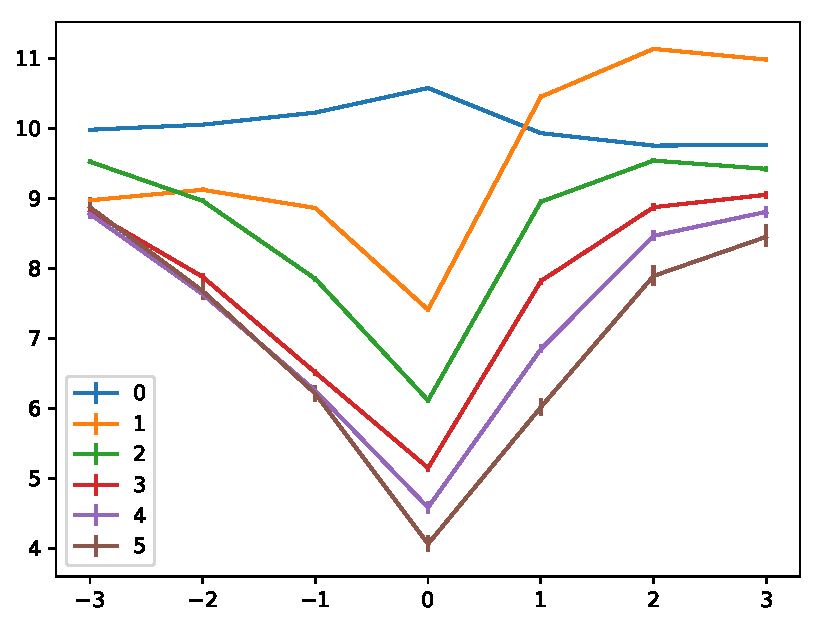
\includegraphics[width=0.4\textwidth]{figures/segmentation-profile-pmis-german-all-heights-ci.pdf}
% %\caption{PMI between left and right contexts, as estimated by the LSTM CNLM in German, organized by syntactic hierarchical distance between subsequent characters (with bootstrapped 95 \% confidence intervals).}\label{fig:syntax-depth}
% %\end{figure}
% %
% %
% %
% %%687112
% %%73757
% %%46716
% %%22847
% %7896
% %2587
% %827
% %234
% %80





% %
% %
% %
% %% (whitespace), if it is distilling meaningful linguistic knowledge, we
% %% expect that it should develop some implicit notion of word-like units.
% %Early work on word segmentation has shown that low transition
% %probabilities \cite{harris-distributional-1954, saffran-word-1996},
% %high uncertainty about the next character \cite{cohen-algorithm-2001,
% %  feng-accessor-2004} and low mutual information
% %\cite{sun-chinese-1998} serve as statistical cues to word
% %segmentation.  %In Figure~\ref{fig:syntax-depth}, we plot (1) entropy
% %% of the predicted distribution over the next character around word
% %% boundaries, compared to other positions, and (2) the pointwise mutual
% %% information (PMI) between left and right contexts, computed by
% %% subtracting the unconditional log-likelihood of the next 20 characters
% %% from their log-likelihood conditioned on the prior context, both computed
% %% using our pre-trained LSTM on a section of the German training
% %% set.  We see that higher entropy and lower PMI computed on
% %% model-generated probabilities correlate with word boundaries,
% %% suggesting that the model internalized statistics that cue segmentation.
% %%
% %% \begin{figure}
% %% 	\begin{center}
% %% 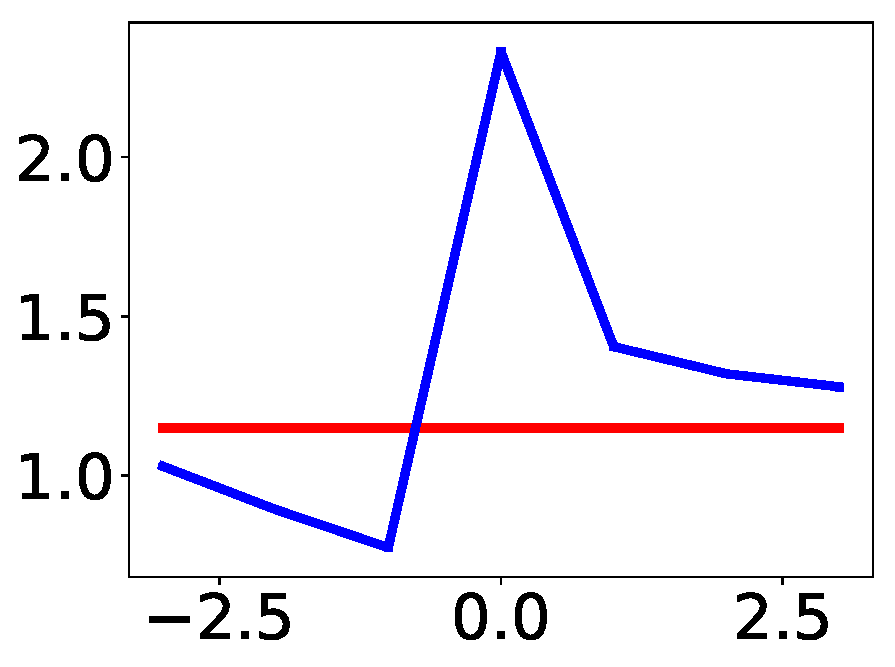
\includegraphics[width=0.22\textwidth]{figures/segmentation-profile-flattened-entropies-english-ci.pdf}
% %% 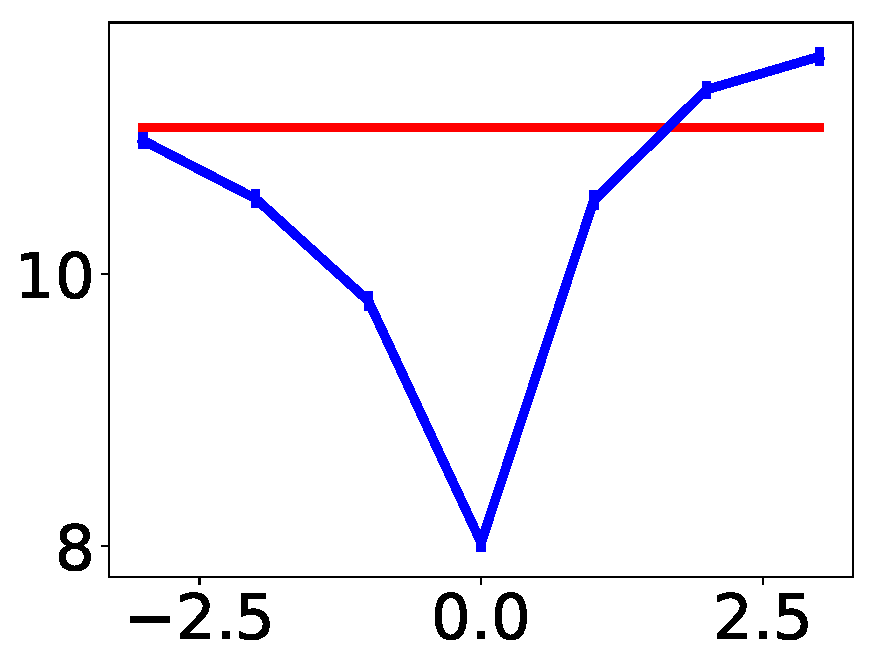
\includegraphics[width=0.22\textwidth]{figures/segmentation-profile-flattened-pmis-english-ci.pdf}
% %% 	\end{center}
% %% 	\caption{Average entropy over the next character (left) and PMI between left and right contexts (right) around word boundaries (blue); the x-axis indicates position relative to a word boundary. The red line indicates the overall average of the quantity. Error bars indicate (almost imperceptible) bootstrapped 95 \% confidence intervals.}\label{fig:boundaries-entropy}
% %% \end{figure}
% %%
% %Based on these considerations, we tested the model segmentation
% %capabilities as follows. We used the development sets to
% %train  logistic classifiers predicting whether a character is first in
% %a word or not, based on the following features, derived from the
% %pre-trained CNLMs without further tuning: (1) \emph{surprisal}, the
% %log-probability of the character given prior context, (2)
% %\emph{entropy} of the distribution over the character given prior
% %context, (3) \emph{context PMI}, that is, the total
% % likelihood of the next 20 characters, minus the unconditional
% % likelihood estimated by starting the CNLM at the current position. %
% %%The rationale of (3) is that it measures the pointwise mutual information, and thus the statistical association, between the subsequent characters and the prior context, which we hypothesize will be higher inside words.
% %%It is also the transition probability for the next characters
% %%(3) can also be interpreted as the result of normalizi transition probability
% % We collected these quantities for each position and the preceding
% % and following three characters, resulting in a 21-feature classifier. %
% %%In total, the classifier has 21 coefficients.
% %We repeated the  experiment with features extracted from a
% %character-level 8-gram model estimated on the training set, closer to
% % earlier non-neural work
% %\cite{saffran-word-1996, feng-accessor-2004}.
% %
% %
% %\begin{table}[t]
% %	\small
% %  \begin{center}
% %    \begin{tabular}{l|l|l|l}
% %      \multicolumn{1}{c|}{}&\emph{LSTM}&\emph{RNN}&\emph{8-grams}\\
% %      \hline
% %      English & 66/60/63 &   63/60/61 & 56/51/53    \\ % \ldots{}/\ldots{}/\ldots & \ldots{}/\ldots{}/\ldots & \ldots{}/\ldots{}/\ldots &\ldots{}/\ldots{}/\ldots\\
% %      German &  57/52/55 &  53/49/51 & 43/36/39   \\ %   \ldots{}/\ldots{}/\ldots & \ldots{}/\ldots{}/\ldots & \ldots{}/\ldots{}/\ldots &\ldots{}/\ldots{}/\ldots\\
% %      Italian &  64/57/60 & 62/57/60  & 48/40/44    \\ % \ldots{}/\ldots{}/\ldots & \ldots{}/\ldots{}/\ldots & \ldots{}/\ldots{}/\ldots &\ldots{}/\ldots{}/\ldots\\
% %    \end{tabular}
% %  \end{center}
% %  \caption{\label{tab:segmentation-results} Percentage precision, recall, and F1 on test set word segmentation.}
% %\end{table}
% %
% %
% %% \begin{table}[t]
% %% 	\footnotesize
% %%   \begin{center}
% %%     \begin{tabular}{l|l|l|l}
% %%       \multicolumn{1}{c|}{}&\emph{LSTM}&\emph{RNN}&\emph{8-grams}\\
% %%       \hline
% %%       English & 65.8/60.4/63.0 &   63.3/59.8/61.5 & 55.7/51.0/53.3    \\ % \ldots{}/\ldots{}/\ldots & \ldots{}/\ldots{}/\ldots & \ldots{}/\ldots{}/\ldots &\ldots{}/\ldots{}/\ldots\\
% %%       German &  57.0/52.5/54.7 &  53.2/49.3/51.1 & 42.9/36.3/39.3   \\ %   \ldots{}/\ldots{}/\ldots & \ldots{}/\ldots{}/\ldots & \ldots{}/\ldots{}/\ldots &\ldots{}/\ldots{}/\ldots\\
% %%       Italian &  63.6/56.9/60.1 & 62.5/57.5/59.9  & 48.4/39.6/43.6    \\ % \ldots{}/\ldots{}/\ldots & \ldots{}/\ldots{}/\ldots & \ldots{}/\ldots{}/\ldots &\ldots{}/\ldots{}/\ldots\\
% %%     \end{tabular}
% %%   \end{center}
% %%   \caption{\label{tab:segmentation-results} Percentage precision, recall, and F1 on test set word segmentation.}
% %% \end{table}
% %
% %%PMI alone 
% %%P 30.56 R 20.61 F 24.61 German
% %%P 32.19 R 20.89 F 25.34 Italian
% %%P 39.37 R 29.45 F 33.69 English
% %%Surprisal alone
% %%P 28.04 R 18.64 F 22.4 German
% %%P 28.76 R 18.31 F 22.38 Italian
% %%P 33.65 R 24.1 F 28.08 English
% %%Entropy alone
% %%P 50.88 R 45.57 F 48.08 German
% %%P 58.44 R 52.09 F 55.08 Italian
% %%P 59.85 R 53.75 F 56.63 English
% %
% %
% %% For each language model and language, we compute how many of the extracted tokens were correct (precision) and how many of the actual tokens were found by the classifier (recall), together with F1.
% %% The goal of this experiment is not to construct a new word segmentation system, but to evaluate how strongly the CNLM's probabilities are indicative of word boundaries.
% %
% %Results are in Table~\ref{tab:segmentation-results}. The
% %CNLM-based classifiers robustly segment more than half of the tokens
% %correctly, and do considerably better than the 8-gram model,
% %with a slight edge for the LSTM.%  Ablation shows that entropy is most
% %% predictive, reaching an F1 of 56.6\% (English), 48.1\% (German),
% %% 55.1\% (Italian) on its
% %% own. Surprisal reaches 28.08 (English), 22.4 (German),
% %% 22.38 (Italian); PMI reaches 33.69 (English), 24.61 (German), 25.34
% %% (Italian).  Setting N to other values shows that larger values of N
% %% increase performance (N =10: 62.45, N=20: 63.24).
% %
% %How does the LSTM compare to \emph{ad-hoc} word segmentation models?
% %We look at the Bayesian bigram model of
% %\newcite{goldwater-bayesian-2009}, an elegant approach using a
% %hierarchical Dirichlet process.  The latter, unlike our method, is
% %unsupervised, but it has a specifically designed built-in bias towards
% %a discrete lexicon with a power-law frequency distribution. Note that,
% %while supervised, our model is rather parameter-lean, consisting in a
% %logistic classifier trained on 21 features.
% %%Moreover, unlike standard supervised word segmentation methods, our
% %%classifier does not have direct access to character strings; instead,
% %%it evaluates how strongly quantities computed by the CNLM
% %%\emph{correlate} with word boundaries. \textbf{Not sure I got the
% %%  latter point.}
% %
% %Running Bayesian methods on Wikipedia dumps is computationally
% %unfeasible. We re-trained instead the LSTM (with fixed
% %hyperparameters) on the Brent corpus of English child-directed speech
% %\cite{brent-efficient-1999} also used by Goldwater and colleagues.  We
% %used 90\% to train our language model, 5\% to fit the logistic
% %classifier, and 5\% for evaluating both the classifier and the Bayesian model on word segmentation.
% %The Bayesian
% %model is trained %and evaluated
% %on the full data-set, as it does not
% %rely on word boundary information during training. Results in
% %Table~\ref{tab:segmentation-results-brent} show that the CNLM
% %performance is comparable to that of the sophisticated Bayesian
% %segmentation method.
% %%\footnote{We found very similar results when
% %%testing the Bayesian model only on the subset used to test  our logistic classifier.}
% %
% %% \begin{table*}[t]
% %%   \begin{center}
% %%     \begin{tabular}{ll|l|l|l|l}
% %%       \multicolumn{2}{c|}{}&Tokens & Lexical & Boundaries\\      \hline
% %% 	    \multirow{4}{*}{CNLM} & Full model & 0.75/0.76/0.75 & 0.41/0.61/0.49 & 0.91/0.90/0.90 \\
% %% 	    &     log-probability & 51.0/45.3/48.0 & 48.8/19.5/27.9 & 80.5/71.6/75.8 \\
% %% 	    &     entropy & 50.4/53.3/51.8 & 52.0/21.1/30.0 & 79.0/74.7/76.8\\
% %% 	    &     PMI & 70.8/72.9/71.8 & 57.6/34.6/43.2 &89.9/87.3/88.6  \\ \hline
% %% 	    \multicolumn{2}{c|}{\citet{goldwater-bayesian-2009}} & 75.2/69.6/72.3 & 63.5/55.2/59.1 & 90.3/80.8/85.2
% %%     \end{tabular}
% %%   \end{center}
% %% 	\caption{\label{tab:segmentation-results-brent} Word segmentation results (percentage precision/recall/F1)  on the Brent corpus for our CNLM-based model and the Bayesian approach of \cite{goldwater-bayesian-2009}. Following \cite{goldwater-bayesian-2009}, we evaluate at the level of tokens, the lexicon of induced word types, and boundaries.}
% %% \end{table*}
% %
% %
% %%\begin{table}[t]
% %%  \begin{small}
% %%    \begin{center}
% %%      \begin{tabular}{l|ll}
% %%        &	     LSTM & Bayesian \\ \hline %\citet{goldwater-bayesian-2009} \\ \hline
% %%        Tokens & 75.3/76.6/76.0 & 75.2/69.6/72.3 \\
% %%        Lexical & 41.2/61.2/49.2 &63.5/55.2/59.1  \\
% %%        Boundaries & 91.3/90.0/90.5 & 90.3/80.8/85.2 \\
% %%      \end{tabular}
% %%    \end{center}
% %%  \end{small}
% %%  \caption{\label{tab:segmentation-results-brent} Word segmentation results (percentage precision/recall/F1)  on the Brent corpus for our CNLM-based model and the Bayesian approach of \newcite{goldwater-bayesian-2009}. Following them, we evaluate at the level of tokens, the lexicon of induced word types, and boundaries.}
% %%\end{table}
% %%
% %
% %\begin{table}[t]
% %  \begin{small}
% %    \begin{center}
% %      \begin{tabular}{l|ll}
% %        &	     LSTM & Bayesian \\ \hline %\citet{goldwater-bayesian-2009} \\ \hline
% %        Tokens & 75.3/76.6/76.0 & 74.9/69.8/72.3 \\
% %        Lexical & 41.2/61.2/49.2 & 63.6/60.2/61.9 \\
% %        Boundaries & 91.3/90.0/90.5 & 93.0/86.7/89.8 \\
% %      \end{tabular}
% %    \end{center}
% %  \end{small}
% %  \caption{\label{tab:segmentation-results-brent} Word segmentation results (percentage precision/recall/F1) on our test partition of the Brent corpus for our CNLM-based model and the Bayesian approach of \newcite{goldwater-bayesian-2009}. Following them, we evaluate at the level of tokens, the lexicon of induced word types, and boundaries.}
% %\end{table}
% %
% %
% %
% %%\begin{table*}[t]
% %%  \begin{center}
% %%    \begin{tabular}{l|l|l|l|l}
% %%      &Tokens & Lexical & Boundaries\\      \hline
% %%	    CNLM & 75.3/76.6/76.0 & 41.2/61.2/49.2 & 91.3/90.0/90.5 \\
% %%	    \citet{goldwater-bayesian-2009} & 75.2/69.6/72.3 & 63.5/55.2/59.1 & 90.3/80.8/85.2
% %%    \end{tabular}
% %%  \end{center}
% %%	\caption{\label{tab:segmentation-results-brent} Word segmentation results (percentage precision/recall/F1)  on the Brent corpus for our CNLM-based model and the Bayesian approach of \newcite{goldwater-bayesian-2009}. Following them, we evaluate at the level of tokens, the lexicon of induced word types, and boundaries.}
% %%\end{table*}
% %
% %% As a final piece of evidence that the CNLM has internalized a notion
% %% of word, we trained logistic classifiers directly on the hidden states
% %% of the Wikipedia-trained CNLMs. We achieved accuracy above 90\% (and
% %% always above an n-gram-count-based baseline) for all languages, on the
% %% task of classifying word boundaries in unseen words.
% %
% %%In contrast to the Wikipedia experiments, PMI emerges as the most important predictor on this dataset.
% %
% %word segmentation probing task:
% %
% %- LSTM, RNN probing
% %
% %
% %We looked at common errors made by the English CNLM-based segmenter. Considering first the 30 most common undersegmentations
% %in the test set (that is, cases in which the model failed to split two
% %or more words): About half (16) are function word
% %sequences that could reasonably be re-analyzed as single words (e.g.,
% %\emph{more than}, \emph{as well as}, \emph{such as}). Of the remaining
% %cases, 8 follow the \emph{N of} pattern, where \emph{N} is a
% %(typically relational) noun commonly occurring in this construction
% %(\emph{member of}, \emph{end of}, \emph{part of}\ldots). There are 3
% %fixed multi-word expressions (\emph{New York}, \emph{United States}
% %and \emph{high school}). The final undersegmentations \emph{based on}, \emph{known as} and
% %\emph{according to} can be seen as lexicalized connectives,
% %especially in the Wikipedia text the model was trained on.
% %
% %The picture is murkier but still fairly linguistically grounded
% %for the 30 most common oversegmentation errors (that is, character
% %fragments that are wrongly segmented from inside the largest number of
% %distinct words).\footnote{We ignore here single-letter segmentations,
% %  that would otherwise account for one third of the most-frequent
% %  set.}  More than half (17) are common affixes (prefixes such as
% %\emph{re} and \emph{de} or suffixes such as \emph{ing} and
% %\emph{ly}). 3 strings identical to frequent
% %function words were wrongly carved out of longer words (\emph{the},
% %\emph{to} and \emph{on}). %
% %% , although the model might be treating the
% %% latter as a pseudo-suffix in forms such as \emph{Peterson} and
% %% \emph{Creighton}).
% %The strings \emph{land} and \emph{man} are not unreasonably segmented
% %out of compounds. It's hard to find a linguistically sound motivation
% %for the 8 remaining top oversegmentations, that are, intriguingly, all CV
% %syllables (\emph{la, le, ma, na, ra, ro, se, ta}).
% %
% %% To conclude, we reiterate that knowledge about word segmentation is
% %% only implicit in our CNLM, and indeed the same CNLM-generated cues we
% %% relied upon to build our classifier above are actually tracking
% %% boundaries between linguistic constituents of different depth.


